
%
%  void-input - easy report template for included file
%  EDIT THE LINE ABOVE FOR DOCUMENTATION OF THIS FILE, then delete this line! 
%         

%

% ============================================================
% --- texstudio magic comment: 
% !TEX encoding = UTF-8
% !TeX program = pdflatex
%% !TeX program = xelatex
% !TeX root = "cognome-tesina.tex"
% %  !TeX spellcheck = en_US
% !TeX spellcheck = it_IT


% ====================================================================


\chapter{Task 1}
The first task was not complicated. I managed to implement the 2 sliders easily. and apart from a small confusion problem with the variables, which caused the second slider to change the same values as the first. Fixed this bug everything worked fine. The Figure  \ref{fig:1b} shows the image with the 2 sliders.

\begin{figure}[h]
	\centering
	\begin{minipage}{1\textwidth}
		\centering
		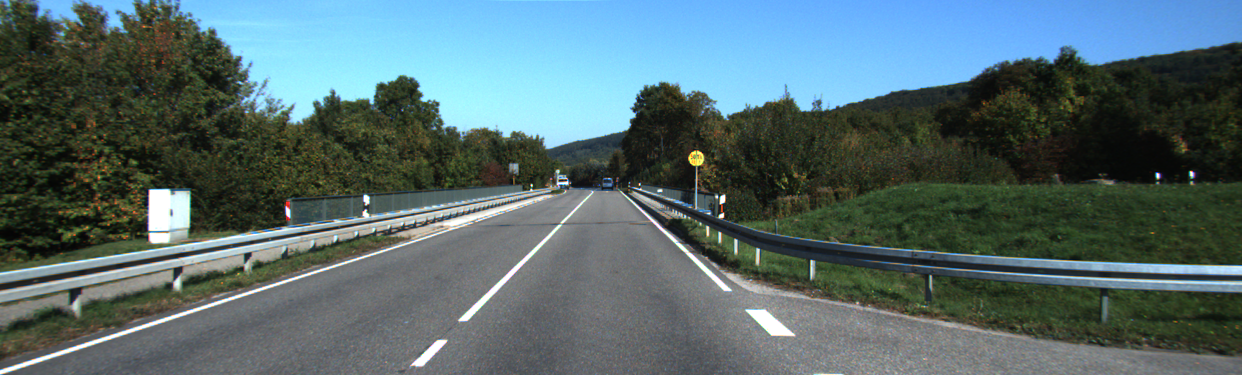
\includegraphics[width=\linewidth]{images/source/0}
		\caption{Original Image.}
		\label{fig:1a}
        \end{minipage}
\end{figure}

\begin{figure}[h]
	\centering
        \begin{minipage}{1\textwidth}
        		\centering
		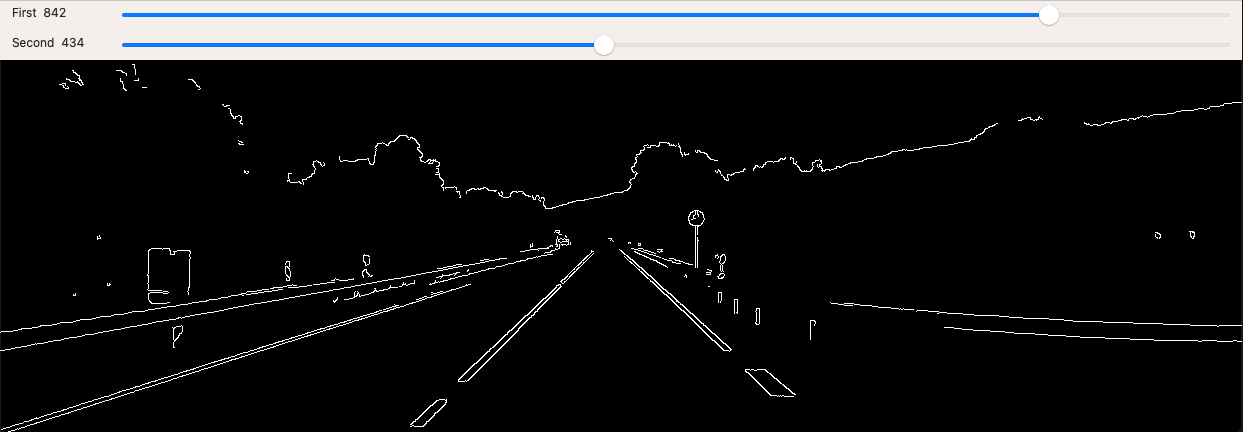
\includegraphics[width=\linewidth]{images/source/task1/1}
		\caption{Edge detection with canny and the sliders.}
		\label{fig:1b}
        \end{minipage}
\end{figure}

\chapter{Task 2}
In this task, the first step of image cannying was not complicated. The second step (i.e. removing unnecessary edges) was more complicated. Without using specific functions to find the lines like cv::HoughLines() and then calculate the slope I didn't know how to do it. Because here I used multiple for loops to clean up the image and finally also to fill the blank lines. I wasted a lot of time looking for "more elegant" solutions than the current one but unfortunately I was unable to do better. Which has very bad time complexity. In Figure  \ref{fig:2a} you can see the image after trimming the canny of excess lines and then the final image in Figure \ref{fig:2b}.

\begin{figure}[h]
	\centering
	\begin{minipage}{0.9\textwidth}
		\centering
		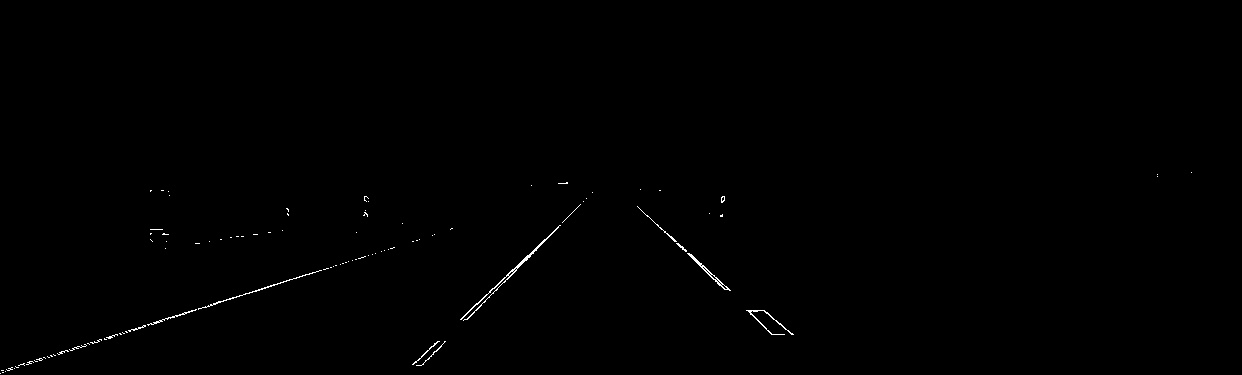
\includegraphics[width=\linewidth]{images/source/task2/1}
		\caption{Edge detection with canny.}
		\label{fig:2a}
        \end{minipage}
\end{figure}

\begin{figure}[h]
	\centering
        \begin{minipage}{0.9\textwidth}
        		\centering
		
\includegraphics[width=\linewidth]{images/source/task2/2}
		\caption{Final result.}
		\label{fig:2b}
        \end{minipage}
\end{figure}


\chapter{Task 3}
After various attempts, including the use of a mask to take only the affected area of the image. I was able to keep only the necessary straight lines thanks to their inclination (Figure \ref{fig:3a}). This allowed me to delimit the edges of the affected area although not with little difficulty. In fact, the lines started from the outside of the image and this made it difficult for me to find the angles that delimited the figure. I used a vector with all the points of the two lines to find the vertices of interest and then thanks to them I traced the image on the main figure (as you can see in the Figure \ref{fig:3b}).

\begin{figure}[h]
	\centering
	\begin{minipage}{1\textwidth}
		\centering
		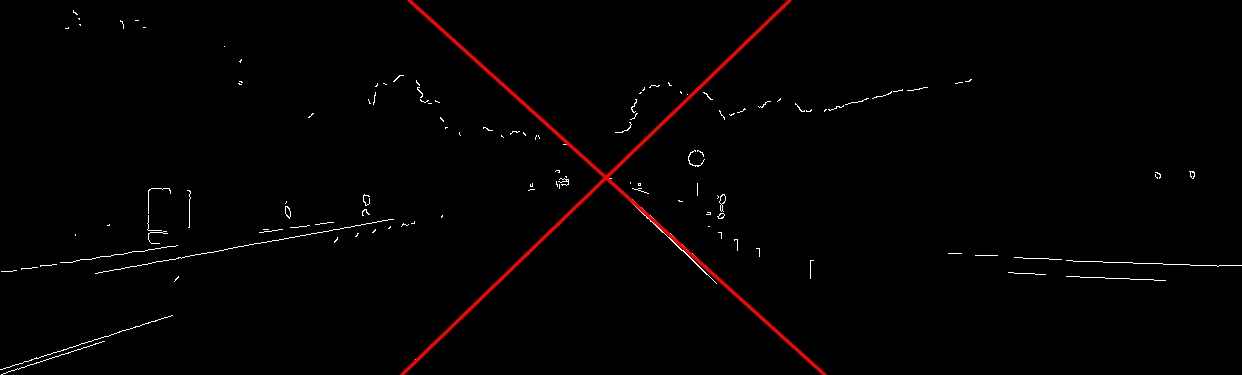
\includegraphics[width=\linewidth]{images/source/task3/1}
		\caption{Image with only the main lines detected with HugeLines.}
		\label{fig:3a}
        \end{minipage}
\end{figure}

\begin{figure}[h]
	\centering
        \begin{minipage}{1\textwidth}
        		\centering
		
\includegraphics[width=\linewidth]{images/source/task3/2}
		\caption{Final image.}
		\label{fig:3b}
        \end{minipage}
\end{figure}

\chapter{Task 4}
The last task was faster than the previous 2 to run although I had some problems using cv::HoughCircles() on the bordered image found by canny. In fact it found circles above it but completely randomly (although it had a low threshold) and when I tried to color them directly in the final image with canny it didn't color them, leaving the image the same as it was immediately after the canny . I fixed it by simply using the grayscale image and directly printing the circles on the color image. In Figure \ref{fig:4a} you can see the final result.

\begin{figure}[h]
	\centering
        \begin{minipage}{1\textwidth}
        		\centering
		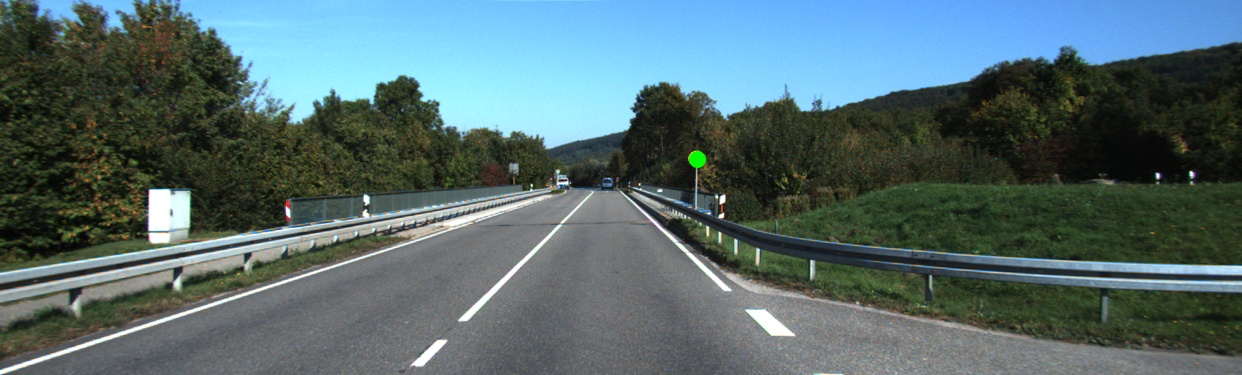
\includegraphics[width=\linewidth]{images/source/task4/1}
		\caption{Final image.}
		\label{fig:4a}
        \end{minipage}
\end{figure}





% ====================================================================

% ====================================================================
% memo available commands
% ====================================================================
% easyrep: summary of provided macros
%
% \Title{text}     defines the document title 
% \Subtitle{text}  defines the subtitle
% \Author{text}    defines the author string
% \Date{text}      defines a date string
% \printCover      print a cover page using above information
%
% --- text styles
% \tDef{text}      definition (generic) 
% \tDefObj{text}   definition (the ter being defined)
% \tDefTxt{text}   definition (the statement defining the term) 
% \tRemark{text}   remarked text
% \tREMARK{text}   highly remarked text 
% \tLoud{text}     shouted text! 
% \tCode{text}     inline code text
% \tLatin{text}    latin text
% \tForeign{text}  foreign language text 
% \tExample{text}  example 
% \tStandard{text} a recommendation 
% \tQuote{text}    a quoted text 
% \tQuoteFig{text} a quoted text referring to a figure 
% \tConcept{text}  an important concept  
% \tBeginPar{text} highlighted text 
%                  at the beginning of a paragraph 
%
% ---environments
% \begin{quoteStandard} text... \end{quoteStandard}
%    print text to be quoted, e.g. sentences from 
%    a recommendation
%
% \begin{quoteRemark} text... \end{quoteRemark}
%    similar to quoteStandrd, but the text is more marked
%
%  
% --- typo accelerators
% \qmo             opening quotation mark (use \qmo{})
% \qmc             closing quotation mark (use \qmc{})
% \th  emphasises "th"
% \ie  slanted "i.e."
% \eg  slanted "e.g."
% \es  slanteg "ad es."
% \octave   "octave" in \tCode style
% \matlab   "matlab"
% \labview  "labVIEW"
% \latex    "LaTeX" (just the text!)
%
% --- math typo accelerators
% \v{math text}  underlines the math text (useful for vector) 
%
% --- debug commands
% \debugTextStyles        print a table showing text styles
% \debugPrintCharacters   print a table of characters
% \Vispa                  print some text (to fill)  
% \Vispas                 more filling text
% ====================================================================
